\let\negmedspace\undefined
\let\negthickspace\undefined

\documentclass[journal,12pt,onecolumn]{IEEEtran}
%\documentclass[journal,12pt,twocolumn]{IEEEtran}
%
\usepackage{setspace}
\usepackage{gensymb}
%\doublespacing
\singlespacing

%\usepackage{graphicx}
%\usepackage{amssymb}
%\usepackage{relsize}
\usepackage[cmex10]{amsmath}
%\usepackage{amsthm}
%\interdisplaylinepenalty=2500
%\savesymbol{iint}
%\usepackage{txfonts}
%\restoresymbol{TXF}{iint}
%\usepackage{wasysym}
\usepackage{amsthm}
\usepackage{mathrsfs}
\usepackage{txfonts}
\usepackage{stfloats}
\usepackage{cite}
\usepackage{cases}
\usepackage{subfig}
%\usepackage{xtab}
\usepackage{longtable}
\usepackage{multirow}
%\usepackage{algorithm}
%\usepackage{algpseudocode}
\usepackage{enumitem}
\usepackage{mathtools}
\usepackage{tikz}
\usepackage{circuitikz}
\usepackage{verbatim}
\usepackage{hyperref}
%\usepackage{stmaryrd}
\usepackage{tkz-euclide} % loads  TikZ and tkz-base
%\usetkzobj{all}
\usepackage{listings}
\usepackage{color}                                            %%
\usepackage{array}                                            %%
\usepackage{longtable}                                        %%
\usepackage{calc}                                             %%
\usepackage{multirow}                                         %%
\usepackage{hhline}                                           %%
\usepackage{ifthen}                                           %%
%optionally (for landscape tables embedded in another document): %%
\usepackage{lscape}     
\usepackage{multicol}
\usepackage{chngcntr}
\usepackage{iftex}
%\usepackage[latin9]{inputenc}
\usepackage{geometry}
\usepackage{bm}
%\geometry{verbose,tmargin=2cm,bmargin=3cm,lmargin=1.8cm,rmargin=1.5cm,headheight=2cm,headsep=2cm,footskip=3cm}
\usepackage{array}
\newcolumntype{L}[1]{>{\raggedright\let\newline\\\arraybackslash\hspace{0pt}}m{#1}}
\newcolumntype{C}[1]{>{\centering\let\newline\\\arraybackslash\hspace{0pt}}m{#1}}
\newcolumntype{R}[1]{>{\raggedleft\let\newline\\\arraybackslash\hspace{0pt}}m{#1}}

%\usepackage{graphicx}
%\usepackage{setspace}
%\usepackage{parskip}

\def \hsp {\hspace{3mm}}

\makeatletter

\providecommand{\tabularnewline}{\\}



\makeatother
\ifxetex
\usepackage[T1]{fontenc}
\usepackage{fontspec}
%\setmainfont[ Path = fonts/]{Sanskrit_2003.ttf}
\newfontfamily\nakulafont[Script=Devanagari,AutoFakeBold=2,Path = fonts/]{Nakula}
%\newfontfamily\liberationfont{Liberation Sans Narrow}
%\newfontfamily\liberationsansfont{Liberation Sans}
\fi
\usepackage{tikz}
\usepackage{xcolor}
%\usepackage{enumerate}

%\usepackage{wasysym}
%\newcounter{MYtempeqncnt}
\DeclareMathOperator*{\Res}{Res}
%\renewcommand{\baselinestretch}{2}
\renewcommand\thesection{\arabic{section}}
\renewcommand\thesubsection{\thesection.\arabic{subsection}}
\renewcommand\thesubsubsection{\thesubsection.\arabic{subsubsection}}

\renewcommand\thesectiondis{\arabic{section}}
\renewcommand\thesubsectiondis{\thesectiondis.\arabic{subsection}}
\renewcommand\thesubsubsectiondis{\thesubsectiondis.\arabic{subsubsection}}

% correct bad hyphenation here
\hyphenation{op-tical net-works semi-conduc-tor}
\def\inputGnumericTable{}                                 %%

\lstset{
	language=tex,
	frame=single, 
	breaklines=true
}

%\begin{document}
%


\newtheorem{theorem}{Theorem}[section]
\newtheorem{problem}{Problem}
\newtheorem{proposition}{Proposition}[section]
\newtheorem{lemma}{Lemma}[section]
\newtheorem{corollary}[theorem]{Corollary}
\newtheorem{example}{Example}[section]
\newtheorem{definition}[problem]{Definition}
%\newtheorem{thm}{Theorem}[section] 
%\newtheorem{defn}[thm]{Definition}
%\newtheorem{algorithm}{Algorithm}[section]
%\newtheorem{cor}{Corollary}
\newcommand{\BEQA}{\begin{eqnarray}}
	\newcommand{\EEQA}{\end{eqnarray}}
\newcommand{\define}{\stackrel{\triangle}{=}}
\bibliographystyle{IEEEtran}
%\bibliographystyle{ieeetr}
\providecommand{\mbf}{\mathbf}
\providecommand{\pr}[1]{\ensuremath{\Pr\left(#1\right)}}
\providecommand{\qfunc}[1]{\ensuremath{Q\left(#1\right)}}
\providecommand{\sbrak}[1]{\ensuremath{{}\left[#1\right]}}
\providecommand{\lsbrak}[1]{\ensuremath{{}\left[#1\right.}}
\providecommand{\rsbrak}[1]{\ensuremath{{}\left.#1\right]}}
\providecommand{\brak}[1]{\ensuremath{\left(#1\right)}}
\providecommand{\lbrak}[1]{\ensuremath{\left(#1\right.}}
\providecommand{\rbrak}[1]{\ensuremath{\left.#1\right)}}
\providecommand{\cbrak}[1]{\ensuremath{\left\{#1\right\}}}
\providecommand{\lcbrak}[1]{\ensuremath{\left\{#1\right.}}
\providecommand{\rcbrak}[1]{\ensuremath{\left.#1\right\}}}
\theoremstyle{remark}
\newtheorem{rem}{Remark}
\newcommand{\sgn}{\mathop{\mathrm{sgn}}}
\providecommand{\abs}[1]{\left\vert#1\right\vert}
\providecommand{\res}[1]{\Res\displaylimits_{#1}} 
\providecommand{\norm}[1]{\left\lVert#1\right\rVert}
%\providecommand{\norm}[1]{\lVert#1\rVert}
\providecommand{\mtx}[1]{\mathbf{#1}}
\providecommand{\mean}[1]{E\left[ #1 \right]}
\providecommand{\fourier}{\overset{\mathcal{F}}{ \rightleftharpoons}}
%\providecommand{\hilbert}{\overset{\mathcal{H}}{ \rightleftharpoons}}
%\providecommand{\system}{\overset{\mathcal{H}}{ \longleftrightarrow}}
\providecommand{\system}[1]{\overset{\mathcal{#1}}{ \longleftrightarrow}}
\providecommand{\gauss}[2]{\mathcal{N}\ensuremath{\left(#1,#2\right)}}
%
%\newcommand{\solution}[2]{\textbf{Solution:}{#1}}
\newcommand{\solution}{\noindent \textbf{Solution: }}
\newcommand{\cosec}{\,\text{cosec}\,}
\newcommand{\sinc}{\,\text{sinc}\,}
\newcommand{\rect}{\,\text{rect}\,}
\providecommand{\dec}[2]{\ensuremath{\overset{#1}{\underset{#2}{\gtrless}}}}
\newcommand{\myvec}[1]{\ensuremath{\begin{pmatrix}#1\end{pmatrix}}}
\newcommand{\mydet}[1]{\ensuremath{\begin{vmatrix}#1\end{vmatrix}}}
\newcommand*{\permcomb}[4][0mu]{{{}^{#3}\mkern#1#2_{#4}}}
\newcommand*{\perm}[1][-3mu]{\permcomb[#1]{P}}
\newcommand*{\comb}[1][-1mu]{\permcomb[#1]{C}}
%\numberwithin{equation}{section}
\numberwithin{equation}{section}
%\numberwithin{problem}{section}
%\numberwithin{definition}{section}
\makeatletter
\@addtoreset{figure}{problem}
\makeatother
%\let\StandardTheFigure\thefigure
\let\vec\mathbf
%\renewcommand{\thefigure}{\theproblem.\arabic{figure}}
\renewcommand{\thefigure}{\arabic{section}.\arabic{figure}}
%\setlist[enumerate,1]{before=\renewcommand\theequation{\theenumi.\arabic{equation}}
	%\counterwithin{equation}{enumi}
	%\renewcommand{\theequation}{\arabic{subsection}.\arabic{equation}}
\let\StandardTheFigure\thefigure
	\vspace{3cm}
	%\usepackage{babel}
	\begin{document}
		\title{Decision Trees}
		\maketitle
		\author{ Mannem Charan AI21BTECH11019}
		\begin{abstract}
			This report consists of my basic understanding of one of the popular Ml methods "Decision Trees".
		\end{abstract}
                \section{Decision Trees}
                 Decision trees is a supervised machine learning algorithm (where the techniques developed use labelled dataset to classify the data or predict the outcome) used to solve general classification and regression problems.As the name suggests, it uses a tree classifier in which internal nodes represent the features/attributes to be tested and leaf nodes represents the class labels. The method is quite similar to how a normal person do decision making.
                \section{How it is different from Logistic/Linear Regression?}
                 Well as you can see, in logistic/linear regression we are trying to find a best line/curve which fits the data,i.e., we are finding suitable weights which can fit the data. The model starts with assuming that there is linear relationship between independent and dependent variables.The machine learning techniques of this sort are generally known as \textbf{Parametric machine learning algorithms}.This is where the red line comes, Decision trees will not assume any kind of relationship between the independent and dependent variables.These kind of techniques are known as \textbf{"Non-parametric machine learning algorithms"}.
They often used when we don't have any prior knowledge about training data.
                \section{Understanding Decision Trees}
                 As we said earlier, decision trees uses a tree-structured classifier which means at each node we are asked to choose one path/sub-branch, and the decision we make split the tree into sub trees. This process continues until we end up hitting leaf nodes which are nothing but labels.In the decision trees, we need to know some basic terminology, those are 
                \begin{enumerate}
                 \item \textbf{Root node:}The first node that we will encounter in a decision tree,which further divides into many sub trees.
                 \item \textbf{Leaf node:} The leaf nodes are the final nodes, the tree cannot be segregated further after encountering a leaf node.
                 \item \textbf{Decision node:} At each decision node, we are asked to make a decision, according that we will travel through nodes.    
                \end{enumerate}
     To get better idea you can see Fig $\ref{Fig 1}$,
           \begin{figure}
             \centering
             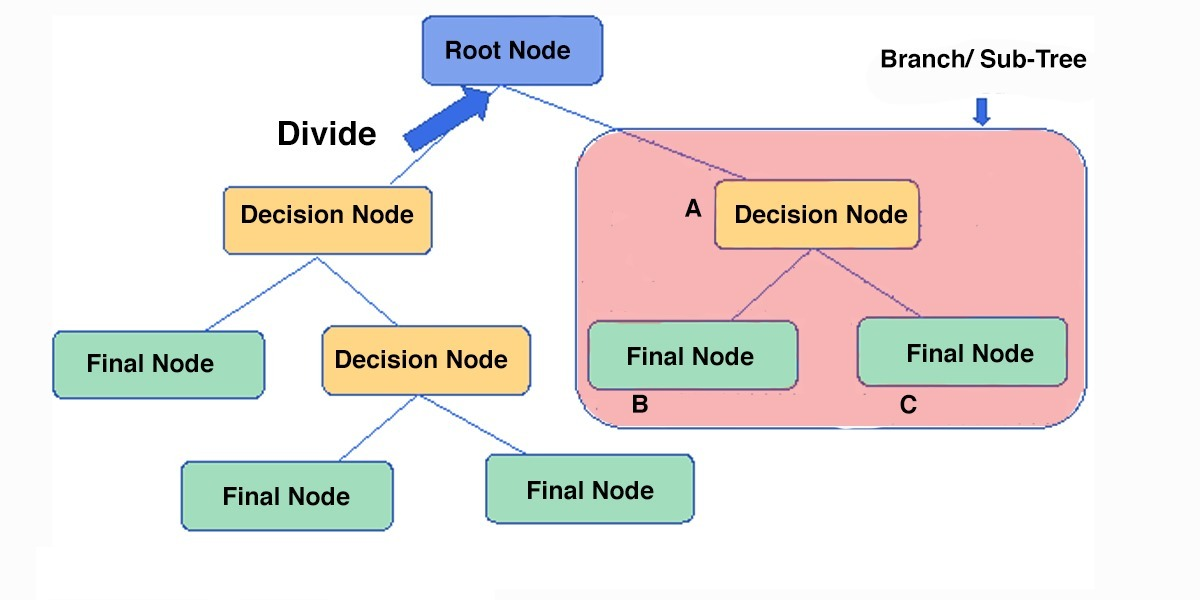
\includegraphics[width = 10cm]{treeexample.png}
             \caption{A tree example}
             \label{Fig 1}
           \end{figure}
     So basically in decision trees each node represents a feature/attribute of the data and the data splits at every node based on the decision we make until we reach the leaf nodes which are basically the labels predicted by decision trees for the data.It is as simply as it sounds but the only task we have here is to construct a proper decision tree since we can't randomly choose an attribute as a root node.The method we are using to select a attribute over other is known as \textbf{"Attribute Selection Measure"}. Now before going to ASM, as we said that it used for Regression it means that labels at leaf nodes are just real numbers so as you might have guessed it can only play some cards when it comes to regression. So it is more preffered for Classification problems than regression.
              \section{Attribute Selection Measure:}
          In Attribute Selection Measure, we will give a value to each attribute, which represents how important/reliable the attribue is to predict the outcome.The value is known as \textbf{"Information Gain"}. Based on this value, the hierarchy of the nodes/attributes is decided.So the attribute with highest information gain will be considered as "root node"and it will be the first split in the tree. Splitting continues until all childeren nodes are \textbf{pure} or the information gain is $0$.
              \subsection{Information Gain}
               Based on the value of information gain we will decide whether some attributes are necessary or not,i.e., we will remove some attribute which has low or $0$ information gain.This process is known as \textbf{"Pruning"}.Now we will see how to calculate information gain,
	    \begin{align}
		    I\brak{T,A} &= S\brak{T} - \sum_{v\in A}\frac{\abs{T_v}}{T}.S\brak{T_v}\label{eq 1}
	    \end{align}
	    where,
	    \begin{itemize}
	      \item T = Target attribute, the feature based on which the data is classified.
              \item A = The attribute choosen to calculate information gain.
	      \item v = The each unique value in A.
              \item S\brak{T} = Entropy of the target attribute. 
            \end{itemize}
       To understand the $\eqref{eq 1}$,first we will see what "Entropy" means in this context.\\
       \textbf{Entropy :} With our prior knowledge, we can say that entropy is degree of randomness.To understand that in this scenario, let us take an example, let say
	we choose 10 persons in that 3 people love anime and 7 people think that it is cartoon. If someone them did they love anime then there will be a "mixed" answers.
	In information theory, entropy gives us a way to quantify this "mixed" thing.It is a measure of how random a data is.If all the 10 people think it is cartoon then the entropy will be $0$ since there is no "mixed" responses.If it is equally distributed then the entropy would be $1$ since there is fair chance for one of them to be true.The entropy is formulated as,
	    \begin{align}
		    S &= -\sum_{i=1}^{c}\pr{X_i}\log_2\pr{X_i}
	    \end{align}
	where,
	\begin{itemize}
         \item The $i$ will iterate over the each unique value in the data.
         \item \pr{X_i} = The probability of the unique value occuring in the data.
        \end{itemize}
	The equation $\eqref{eq 1}$,can also be written as,
	        \begin{align}
			I &= \mathbf{Original\,Entropy}\brak{T} -\mathbf{Weighted\, sum \,of\, Entropies}\brak{T_v}\brak{\text{after\, the\, split}}
		\end{align}
         If $I$ is positive, then overall entropy decreased, which means the randomness is decreased and now we can predict more accurately.So we need check $I$ for every attribute and choose which has more value.
        \subsection{Gini Index}
	 Similar to what we have discussed in entropy,gini index is another measure by which we split the tree based on randomness/impurity(We will also use impure term in place random).The value of gini index ranges from $0$ to $0.5$.The algorithm which used gini index to derive decision trees is known as CART algorithm.\\The gini index can be calculated as,
	   \begin{align}
		   Gini\brak{T} &= 1 - \sum_iP_i^2\brak{T}
	   \end{align}
         where, $T$ is the target attribute.\\
	 Same as in previous case gini index is calculated for every attribute and we will choose the node with lowest gini index.
       \section{Advantages of decision trees}
        \begin{enumerate}
	 \item It is easy to understand as it similar to how a human thinks while making a decision
         \item Since it will not assume any relationship between independent and dependent variables, it can fit for any data.
         \item It is very useful algorithm for decision making
	\end{enumerate}
       \section{Disadvantages of decision trees}
         \begin{enumerate}
	   \item It requires more computation power as the class labels increases.
	   \item Often has overfitting problem.
	 \end{enumerate}
       \section{Questions:}
         \begin{enumerate}
	  \item Explain the structure of Decision trees?
	  \item List out the different techniques used for ASM?
	  \item How to select the root node for decision tree using IG ASM?
	  \item Do we require feature scaling in Decision Trees?
	  \item How can avoid overfitting in Decision trees?
         \end{enumerate}
       \section{Solutions:}
       \begin{enumerate}
         \item Decision tree is tree-like classifier in which,
          \begin{enumerate}
	        \item Each internal node is an attribute and we are being asked to make a decision to go to the child nodes.
		\item Each branch from a internal node represents the decision that you made.
		\item Each leaf node is the class label.
	      \end{enumerate}
	 \item There are two popular techniques used for ASM,
		 \begin{enumerate}
	           \item Using Information Gain and the name of the algorithm is ID3(Iterative Dichotomiser 3).
		   \item Using Gini index and the name of the algorithm is CART(Classification and Regression trees)
		 \end{enumerate}
	 \item The node which has more information gain value will be considered as root node.
	 \item In decision trees, we don't require feature scaling because it is a rule based approach and not sensitive to the variance of the data.
         \item We can avoid overfitting by doing pre-pruning and post-pruning.
                \begin{enumerate}
		\item \textbf{Pre-pruning:}Pruning the branches before generating the decision tree.
		\item \textbf{Post-pruning:} As the name suggests first it will allows the tree to grow to its full depth, then removes the tree branches.
		\end{enumerate}
	 \end{enumerate}
        \end{document}
